\documentclass[12pt]{article}
\usepackage{latexblog}

% ============================================================
% Blog Metadata
% ============================================================
\blogtitle{使用Vagrant来管理Virtualbox}
\blogdate{2019-12-13}
\blogtags{Vagrant, 云计算, 容器化}
\bloglang{zh}
\blogsummary{}

\begin{document}
\makeblogtitle

一直以来我用Virtualbox都是手动创建虚拟机，然后安装操作系统，虽然这个过程本身并不复杂但是也要重复操作和花费时间。通过Vagrant可以像使用Docker一样，编写脚本来管理虚拟机的配置，还可以通过公共的镜像仓库来获取一些别人已经构建好了的镜像。

\section{创建新的虚拟机}\label{ux521bux5efaux65b0ux7684ux865aux62dfux673a}

通过Vagrant有两种方法来创建新的虚拟机：

\begin{itemize}
\tightlist
\item
  使用vagrant命令生成一个Vagrantfile
\item
  手动编写Vagrantfile
\end{itemize}

例如，创建一个ubuntu的镜像，使用\href{https://app.vagrantup.com/ubuntu/boxes/trusty64}{ubuntu/trusty64}这个镜像，可以首先通过如下的命令在当前文件夹下生成一个Vagrantfile：

\begin{Shaded}
\begin{Highlighting}[]
\ExtensionTok{vagrant}\NormalTok{ init ubuntu/trusty64}
\end{Highlighting}
\end{Shaded}

生成的Vagrantfile如下：

\begin{Shaded}
\begin{Highlighting}[]
\ExtensionTok{Vagrant.configure}\ErrorTok{(}\StringTok{"2"}\KeywordTok{)} \ControlFlowTok{do} \KeywordTok{|}\ExtensionTok{config}\KeywordTok{|}
  \ExtensionTok{config.vm.box}\NormalTok{ = }\StringTok{"ubuntu/trusty64"}
\ExtensionTok{end}
\end{Highlighting}
\end{Shaded}

Vagrantfile就相当于Dockerfile，可以定义虚拟机的一些配置，除此之外还可以定义一些其他的参数。然后，要启动它可以这样：

\begin{Shaded}
\begin{Highlighting}[]
\ExtensionTok{vagrant}\NormalTok{ up}
\end{Highlighting}
\end{Shaded}

值得注意的是，截止目前，最新的Virtualbox6.1是不被Vagrant支持的，只能使用6.0.x版本。创建完成之后就可以在Virtualbox的控制页面看到这个虚拟机了。

\begin{figure}
\centering
\pandocbounded{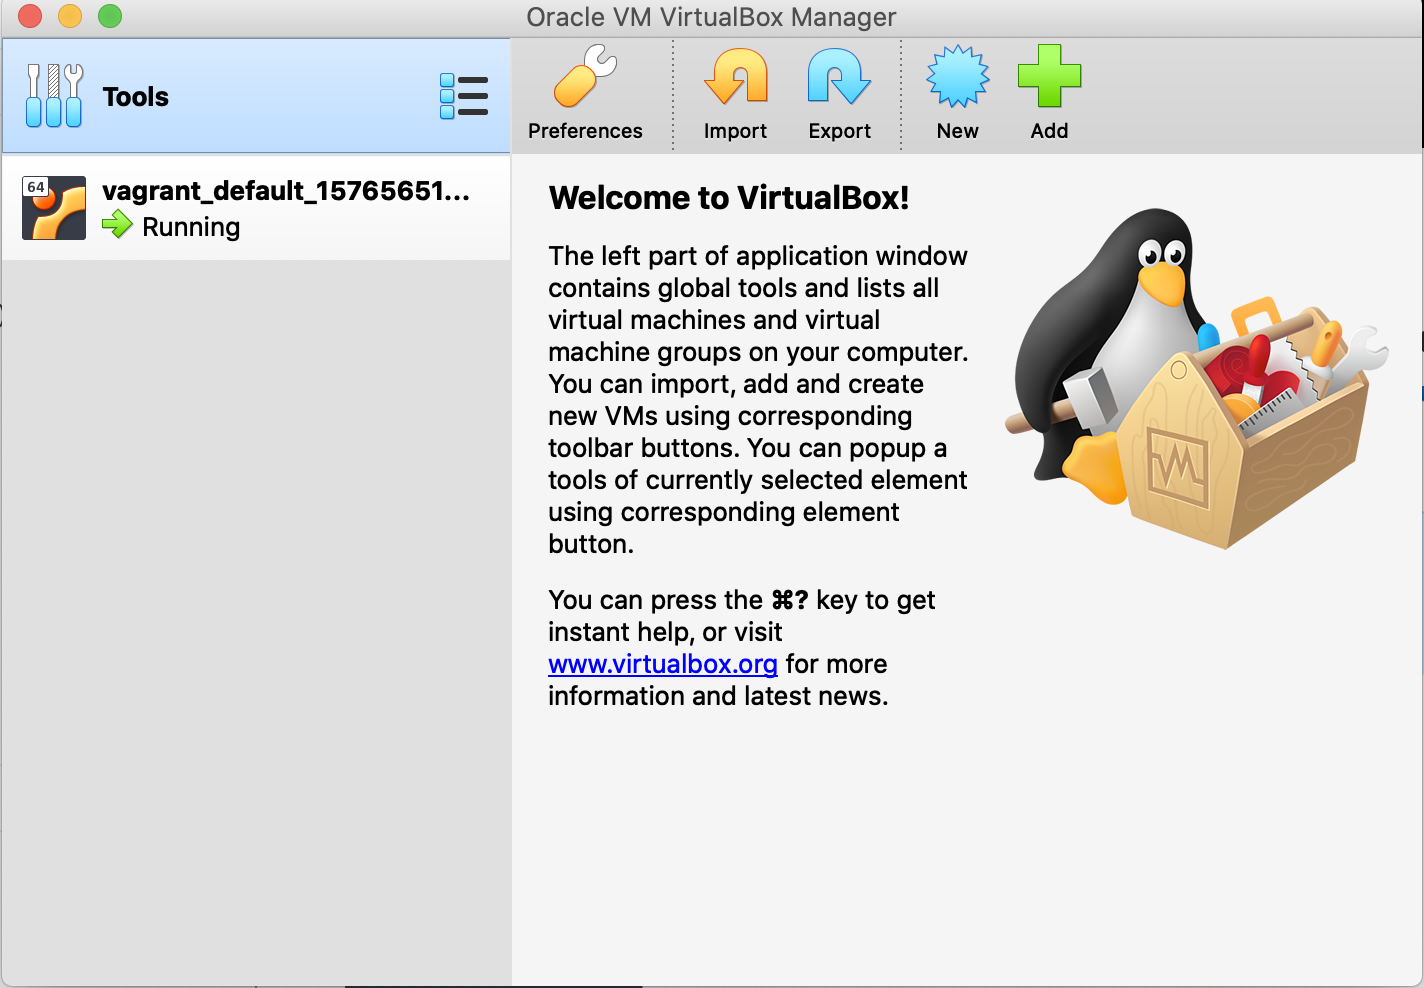
\includegraphics[keepaspectratio,alt={Virtualbox}]{images/Virtualbox.png}}
\caption{Virtualbox}
\end{figure}

\section{解决下载很慢的问题}\label{ux89e3ux51b3ux4e0bux8f7dux5f88ux6162ux7684ux95eeux9898}

有时候


\end{document}
